\documentclass{article}
\iffalse
This file is protected by Copyright. Please refer to the COPYRIGHT file
distributed with this source distribution.

This file is part of OpenCPI <http://www.opencpi.org>

OpenCPI is free software: you can redistribute it and/or modify it under the
terms of the GNU Lesser General Public License as published by the Free Software
Foundation, either version 3 of the License, or (at your option) any later
version.

OpenCPI is distributed in the hope that it will be useful, but WITHOUT ANY
WARRANTY; without even the implied warranty of MERCHANTABILITY or FITNESS FOR A
PARTICULAR PURPOSE. See the GNU Lesser General Public License for more details.

You should have received a copy of the GNU Lesser General Public License along
with this program. If not, see <http://www.gnu.org/licenses/>.
\fi

\author{} % Force author to be blank
%----------------------------------------------------------------------------------------
% Paper size, orientation and margins
%----------------------------------------------------------------------------------------
\usepackage{geometry}
\geometry{
	letterpaper,			% paper type
	portrait,				% text direction
	left=.75in,				% left margin
	top=.75in,				% top margin
	right=.75in,			% right margin
	bottom=.75in			% bottom margin
 }
%----------------------------------------------------------------------------------------
% Header/Footer
%----------------------------------------------------------------------------------------
\usepackage{fancyhdr} \pagestyle{fancy} % required for fancy headers
\renewcommand{\headrulewidth}{0.5pt}
\renewcommand{\footrulewidth}{0.5pt}
\rhead{\small{ANGRYVIPER Team}}
%----------------------------------------------------------------------------------------
% Appendix packages
%----------------------------------------------------------------------------------------
\usepackage[toc,page]{appendix}
%----------------------------------------------------------------------------------------
% Defined Commands & Renamed Commands
%----------------------------------------------------------------------------------------
\renewcommand{\contentsname}{Table of Contents}
\renewcommand{\listfigurename}{List of Figures}
\renewcommand{\listtablename}{List of Tables}
\newcommand{\todo}[1]{\textcolor{red}{TODO: #1}\PackageWarning{TODO:}{#1}} % To do notes
\newcommand{\code}[1]{\texttt{#1}} % For inline code snippet or command line
%----------------------------------------------------------------------------------------
% Various packages
%----------------------------------------------------------------------------------------
\usepackage{hyperref} % for linking urls and lists
\usepackage{graphicx} % for including pictures by file
\usepackage{listings} % for coding language styles
\usepackage{rotating} % for sideways table
\usepackage{pifont}   % for sideways table
\usepackage{pdflscape} % for landscape view
%----------------------------------------------------------------------------------------
% Table packages
%----------------------------------------------------------------------------------------
\usepackage{tabularx} % c=center,l=left,r=right,X=fill
\usepackage{float}
\floatstyle{plaintop}
\usepackage[tableposition=top]{caption}
\newcolumntype{P}[1]{>{\centering\arraybackslash}p{#1}}
\newcolumntype{M}[1]{>{\centering\arraybackslash}m{#1}}
%----------------------------------------------------------------------------------------
% Block Diagram / FSM Drawings
%----------------------------------------------------------------------------------------
\usepackage{tikz}
\usetikzlibrary{shapes,arrows,fit,positioning}
\usetikzlibrary{automata} % used for the fsm
%----------------------------------------------------------------------------------------
% Colors Used
%----------------------------------------------------------------------------------------
\usepackage{colortbl}
\definecolor{blue}{rgb}{.7,.8,.9}
\definecolor{ceruleanblue}{rgb}{0.16, 0.32, 0.75}
\definecolor{drkgreen}{rgb}{0,0.6,0}
\definecolor{deepmagenta}{rgb}{0.8, 0.0, 0.8}
\definecolor{cyan}{rgb}{0.0,0.6,0.6}
\definecolor{maroon}{rgb}{0.5,0,0}
%----------------------------------------------------------------------------------------
% Update the docTitle and docVersion per document
%----------------------------------------------------------------------------------------
\def\docTitle{Component Data Sheet}
\def\docVersion{1.1}
%----------------------------------------------------------------------------------------
\date{Version \docVersion} % Force date to be blank and override date with version
\title{\docTitle}
\lhead{\small{\docTitle}}

\def\comp{agc\_complex}
\def\Comp{AGC Complex}
\graphicspath{ {figures/} }

\begin{document}

\section*{Summary - \Comp}
\begin{tabular}{|c|M{13.5cm}|}
	\hline
	\rowcolor{blue}
	                  &                                                              \\
	\hline
	Name              & \comp                                                        \\
	\hline
	Worker Type       & Application                                                  \\
	\hline
	Version           & v1.1                                                         \\
	\hline
	Release Date      & March 2017                                                   \\
	\hline
	Component Library & ocpi.training.components                                             \\
	\hline
	Workers           & \comp.hdl                                                    \\
	\hline
	Tested Platforms  & xsim, isim, Matchstiq-Z1(PL)(Vivado 2017.1 and ISE 14.7) \\
	\hline
\end{tabular}

\section*{Functionality}
\begin{flushleft}
	The Automatic Gain Control (AGC) Complex component inputs complex signed samples, drives the amplitude of both I and Q input rails to a reference level, and outputs complex signed samples.
\end{flushleft}

	{\centering\captionsetup{type=figure}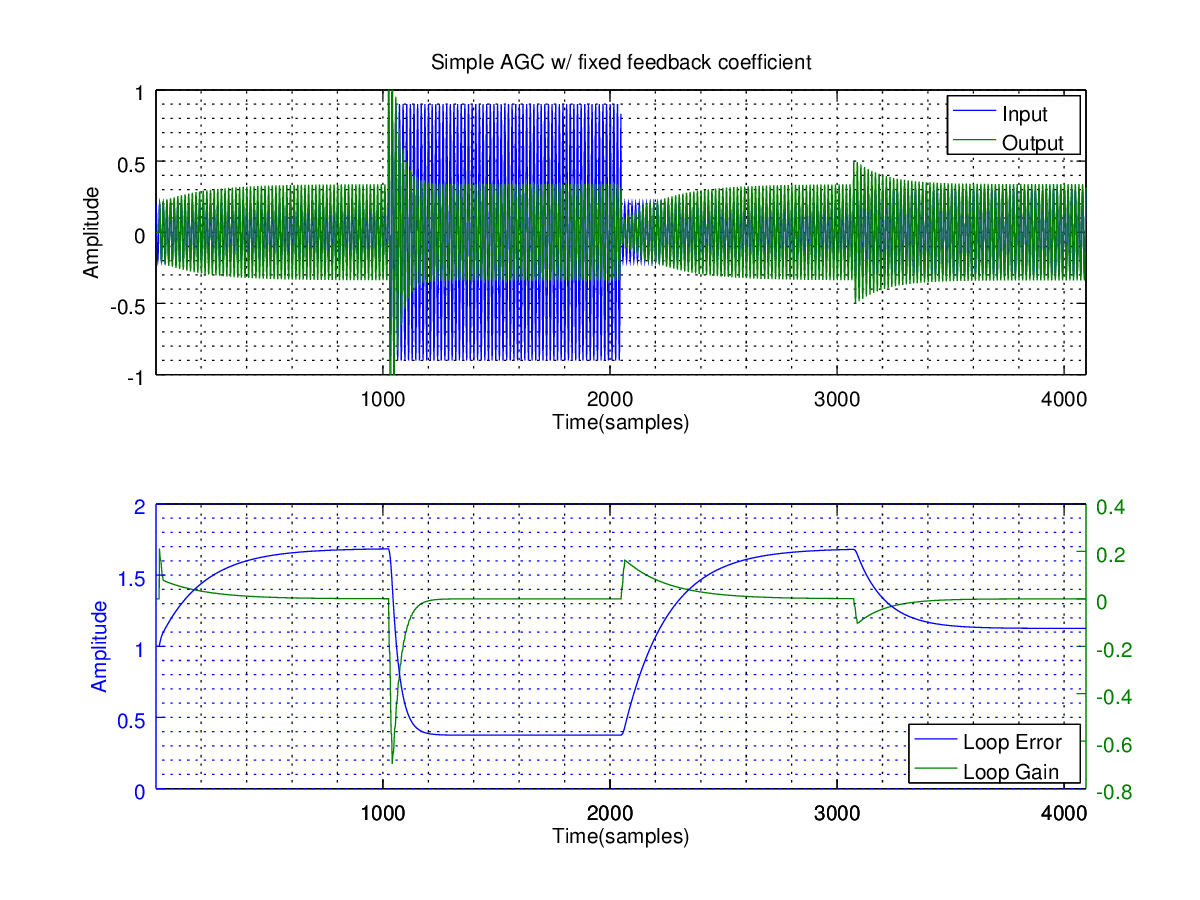
\includegraphics[scale=0.5]{agc_matlab}\par\captionof{figure}{MATLAB AGC implementation with ref=0x1B26 and mu=0x144E}\label{fig:ideal}}

\section*{Worker Implementation Details}
\subsection*{\comp.hdl}
\begin{flushleft}
	The response time and output level of the circuit are programmable, as is the ability to update/hold the gain differential used in the feedback loop. The size of the averaging window used for peak detection is build-time programmable using the \verb+AVG_WINDOW_p+ parameter, which is recommended to be a power-of-two to enable hardware division implementation with shift registers.\medskip

	The \verb+ref+ property controls the desired output amplitude, while the \verb+mu+ property controls the AGC time constant, thus determining the response time of the circuit.\medskip

	This implementation uses three multipliers per I/Q rail to process input data at the clock rate - i.e. this worker can handle a new input value every clock cycle. This circuit will produce output one clock cycle after each valid input, but the input-to-output latency is actually three valid clock cycles.\medskip

	The {\Comp} worker utilizes the OCPI \textit{iqstream\_protocol} for both input and output ports. The \textit{iqstream\_protocol} defines an interface of 16-bit complex signed samples. The \verb+DATA_WIDTH_p+ parameter may be used to reduce the worker's internal data width to less than 16-bits.
\end{flushleft}

\section*{Theory}
\begin{flushleft}
	The circuit is based upon Richard G. Lyons' ``Understanding Digital Signal Processing, Third Edition" Automatic Gain Control (AGC) circuit found on Page 783. The text may also be found online here: \href{http://www.embedded.com/design/other/4214571/A-simple-way-to-add-AGC-to-your-communications-receiver-design-}{DSP-Tricks-A simple way to add AGC to your communications receiver design}. Lyons' circuit in Figure 13-76a implements the AGC function with a feedback loop on y(n) that consists of a magnitude operation to remove the sign, a comparator against the reference level ``ref", a multiplier that uses ``mu" to control the amplitude of the feedback signal (and thus the response time), and finally an accumulator. This implementation uses a peak detector in place of Lyons' simple magnitude operation. From Lyons: ``The process is a nonlinear, time-varying, signal-dependent feedback system. As such, it's highly resistant to normal time-domain or z-domain analysis. This is why AGC analysis is empirical rather than mathematical ..."
\end{flushleft}

\section*{Block Diagrams}
\subsection*{Top level}
\begin{center}
	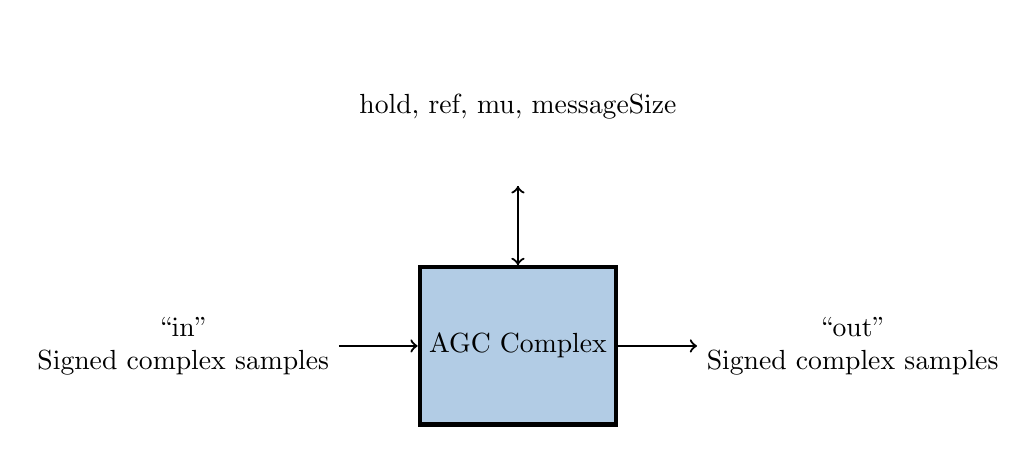
\begin{tikzpicture}[% List of styles applied to all, to override specify on a case-by-case
			every node/.style={
				align=center,  		% use this so that the "\\" for line break works
				minimum size=2cm	% creates space above and below text in rectangle
			},
			every edge/.style={draw,thick}
		]
		\node[rectangle,ultra thick,draw=black,fill=blue](R2){\Comp};
		\node[rectangle,draw=white,fill=white](R3)[left= of R2]{``in" \\ Signed complex samples};
		\node[rectangle,draw=white,fill=white](R4)[right= of R2]{``out" \\ Signed complex samples};
		\node[rectangle,draw=white,fill=white](R5)[above= of R2]{hold, ref, mu, messageSize};
		\path[->]
		(R3)edge []	node [] {} (R2)
		(R2)edge []	node [] {} (R4)
		(R2)edge []	node [] {} (R5)
		(R5)edge []	node [] {} (R2)
		;
	\end{tikzpicture}
\end{center}

\subsection*{State Machine}
\begin{flushleft}
	No finite-state machines (FSM) are implemented by this worker.
\end{flushleft}

\section*{Source Dependencies}
\subsection*{\comp.hdl}
\begin{itemize}
	\item training\_project/components/\comp.hdl/\comp.vhd
	\item training\_project/hdl/primitives/prims/prims\_pkg.vhd
		\subitem training\_project/hdl/primitives/prims/agc/src/agc.vhd
\end{itemize}

\begin{landscape}
	\section*{Component Spec Properties}
		N/A

	\section*{Worker Properties}
	\subsection*{\comp.hdl}
	\begin{scriptsize}
		\begin{tabular}{|c|c|c|c|c|c|c|c|p{6.9cm}|}
			\hline
			\rowcolor{blue}
			Type     & Name                & Type   & SequenceLength & ArrayDimensions & Accessibility       & Valid Range & Default & Usage                                        \\
			\hline
			Property & \verb+DATA_WIDTH_p+ & UShort & -              & -               & Parameter & 1-16        & 16      & Worker internal non-sign-extended data width \\
			\hline
			Property & \verb+AVG_WINDOW_p+ & UShort & -              & -               & Parameter & 4-256       & 16      & Length of the averaging buffer; should be a power of two \\
			\hline
			Property & hold                & Bool   & -              & -               & Writable  & Standard    & false   & Hold disables the gain differential feedback circuit, thus maintaining the current gain \\
			\hline
			Property & ref                 & UShort & -              & -               & Writable  & 1 to $2^{\verb+DATA_WIDTH_p+}-1$ & 0x3FFF & Desired output amplitude expressed in percentage of full scale expected peak value in rms \\
			\hline
			Property & mu                  & UShort & -              & -               & Writable  & 1 to $2^{\verb+DATA_WIDTH_p+}-1$ & N/A & Feedback coefficient used to control the response time of the circuit; expressed as mu*fullscale \\
			\hline
			Property & messageSize         & UShort & -              & -               & Writable  & 8192        & 8192    & Number of bytes in output message                            \\
			\hline
		\end{tabular}
	\end{scriptsize}

	\section*{Component Ports}
	\begin{scriptsize}
		\begin{tabular}{|M{2cm}|M{1.5cm}|M{4cm}|c|c|M{9cm}|}
			\hline
			\rowcolor{blue}
			Name & Producer & Protocol           & Optional & Advanced & Usage                  \\
			\hline
			in   & false    & iqstream\_protocol & false    & -        & Signed complex samples \\
			\hline
			out  & true     & iqstream\_protocol & false    & -        & Signed complex samples \\
			\hline
		\end{tabular}
	\end{scriptsize}

	\section*{Worker Interfaces}
	\subsection*{\comp.hdl}
	\begin{scriptsize}
		\begin{tabular}{|M{2cm}|M{1.5cm}|c|c|M{12cm}|}
			\hline
			\rowcolor{blue}
			Type            & Name & DataWidth & Advanced & Usage                  \\
			\hline
			StreamInterface & in   & 32        & -        & Signed complex samples \\
			\hline
			StreamInterface & out  & 32        & -        & Signed complex samples \\
			\hline
		\end{tabular}
	\end{scriptsize}
\end{landscape}

\section*{Control Timing and Signals}
\begin{flushleft}
	The {\Comp} worker uses the clock from the Control Plane and standard Control Plane signals.
\end{flushleft}

\section*{Performance and Resource Utilization}
\subsubsection*{\comp.hdl}
Table entries are a result of building the worker with the following parameter set:\
\begin{itemize}
	\item \verb+DATA_WIDTH_p+=16
	\item \verb+AVG_WINDOW_p+=16
\end{itemize}
\begin{scriptsize}
	\begin{tabular}{|c|c|c|c|c|c|c|c|}
		\hline
		\rowcolor{blue}
		Device                      & Registers & LUTs & Fmax        & Memory/Special Functions & Design Suite       \\
		\hline
		Zynq XC7Z020-1-CLG484       & 567       & 667  & 229.779 MHz & DSP48E1 = 6              & Vivado 2017.1           \\
		\hline
	\end{tabular}
\end{scriptsize}

\section*{Test and Verification}
\begin{flushleft}
	A single test case is implemented to validate the {\Comp} component. An input file is generated with a single tone at Fs/16 Hz, where Fs = 100 Hz, but applies 20\% of the maximum amplitude to the first quarter of the file, 90\% maximum amplitude to the second quarter of the file, 20\% maximum amplitude to the third quarter of the file, and 30\% maximum amplitude to the fourth quarter of the file. The complex waveform is then scaled to fixed-point signed 16-bit integers. Time and frequency domain plots may be viewed in Figures \ref{fig:in_time_tone} and \ref{fig:in_freq_tone} below, respectively.
\end{flushleft}

	\begin{figure}[ht]
		\centering
		\begin{minipage}{.5\textwidth}
			\centering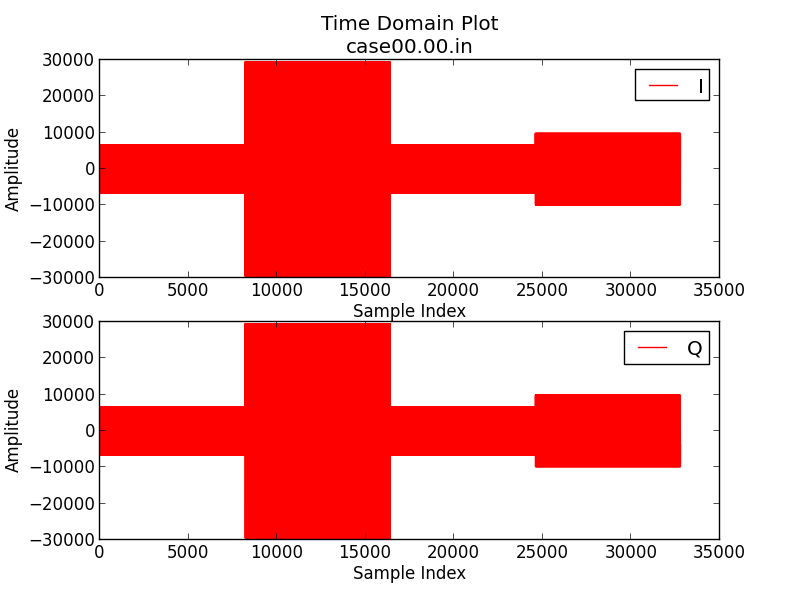
\includegraphics[width=1.0\linewidth]{input_time}
			\captionof{figure}{Time Domain Tone}
			\label{fig:in_time_tone}
		\end{minipage}%
		\begin{minipage}{.5\textwidth}
			\centering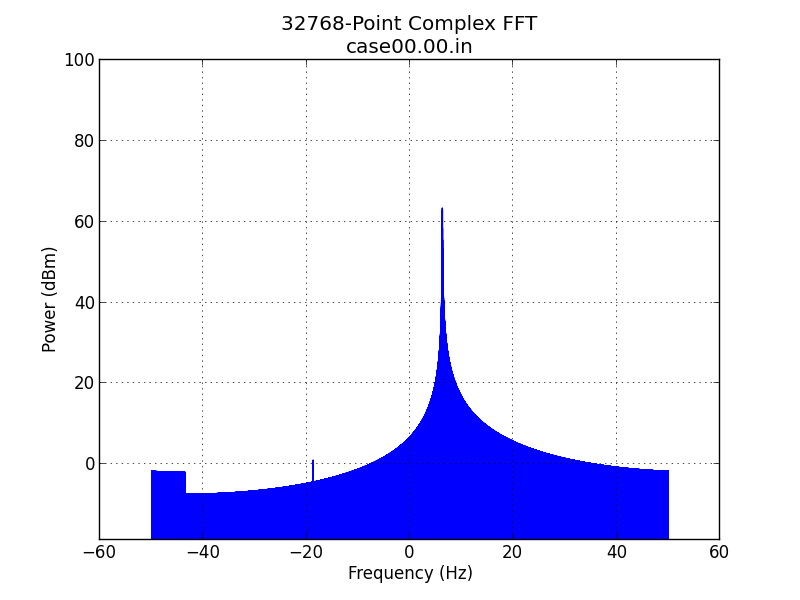
\includegraphics[width=1.0\linewidth]{input_freq}
			\captionof{figure}{Frequency Domain Tone}
			\label{fig:in_freq_tone}
		\end{minipage}
	\end{figure}

\begin{flushleft}
	For verification, the output file is first checked that the data is not all zero, and is then checked for the expected length of 32,768 complex samples. Once these quick checks are made a floating-point python implementation of the AGC is performed on the input data, which is then compared sample-by-sample to the output data. Figures \ref{fig:out_time_tone} and \ref{fig:out_freq_tone} depict the output of the {\Comp} worker.
\end{flushleft}
\newpage

	\begin{figure}[ht]
		\centering
		\begin{minipage}{.5\textwidth}
			\centering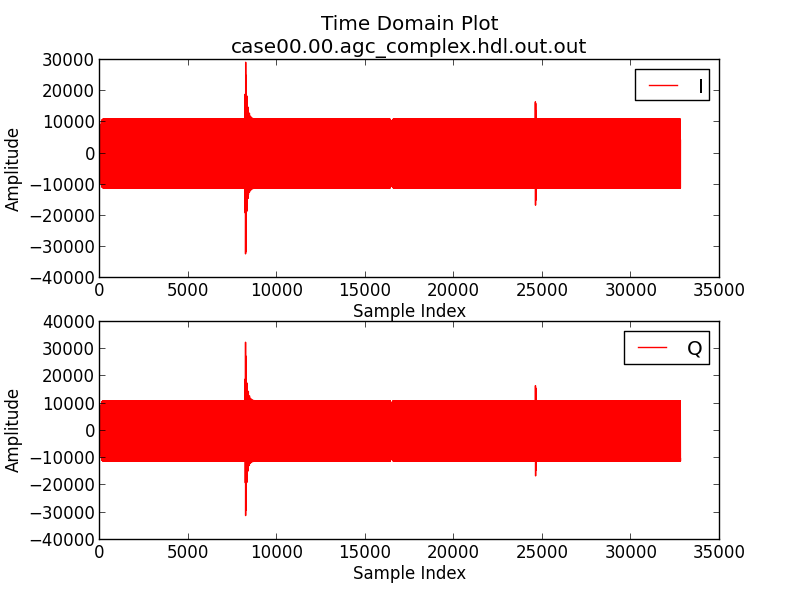
\includegraphics[width=1.0\linewidth]{output_time}
			\captionof{figure}{Time Domain Tones with AGC}
			\label{fig:out_time_tone}
		\end{minipage}%
		\begin{minipage}{.5\textwidth}
			\centering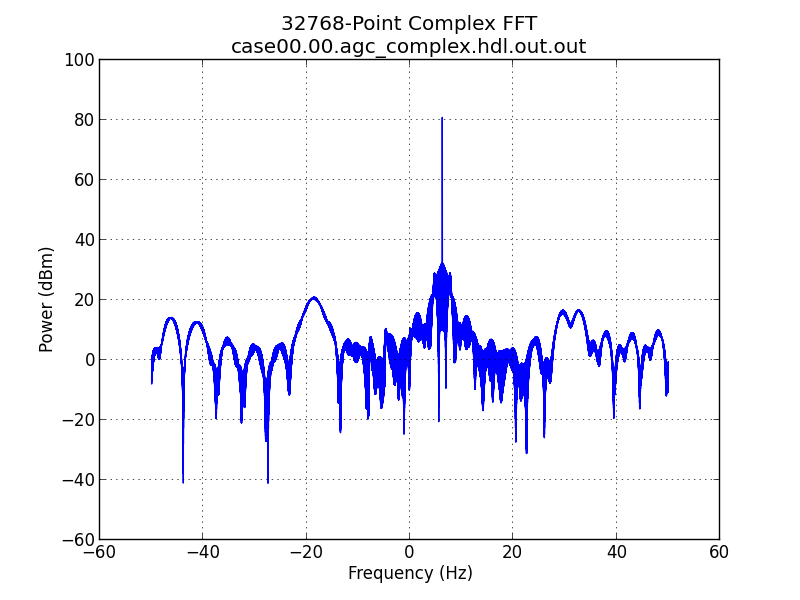
\includegraphics[width=1.0\linewidth]{output_freq}
			\captionof{figure}{Frequency Domain Tones with AGC}
			\label{fig:out_freq_tone}
		\end{minipage}
	\end{figure}

\section*{References}
(1) Richard G. Lyons. \textit{Understanding Digital Signal Processing.} Third Edition. Pearson Education, Inc., Boston. 2001. \\
(2) Richard G. Lyons. (2011, March 29). \textit{A simple way to add AGC to your communications receiver design.} Retrieved from http://www.embedded.com/design/other/4214571/A-simple-way-to-add-AGC-to-your-communications-receiver-design-.

\end{document}
